\documentclass{article}
\usepackage{pedramnotes}

\title{Policy Gradient}
\author{Pedram Rabiee}

\begin{document}


\begin{titlepage}
\thispagestyle{empty}
\maketitle

\tableofcontents


Remaining:
From the Policy Gradient Lecture:
\begin{itemize}
    \item Policy Gradient Implementation
    \item Natural Policy Gradient
\end{itemize}
\end{titlepage}

\newgeometry{top=20mm,bottom=25mm,right=20mm,left=20mm}


\section{Introduction}
The policy gradient methods target at modeling and optimizing the policy directly. The policy is modeled with a parameterized function with respect to $\theta$
\begin{equation*}
    \pi(a \mid s,\theta) = \pi_\theta(a \mid s) = P\{A_t = a \mid S_t = s,\theta_t = \theta\}.
\end{equation*}
The objective is to maximize some performance measure $J(\theta)$
\begin{align*}
    \theta^* &= \argmax_\theta J(\theta)\\
    \theta &\gets \theta + \alpha \nabla_\theta J(\theta)
\end{align*}
To ensure exploration we generally require that the policy never becomes deterministic.

\subsection{Why Policy Gradient?}
\textbf{Advantages}
\begin{itemize}
    \item Better convergence properties.
    
    \item Effective in high-dimensional (there is no need to use maximization) or continuous action spaces.
    
    \item Can learn stochastic policies. In some problems, the optimal policy is stochastic policy (non-Markovian, aliased state). There is always an optimal deterministic policy for a given MDP, that's for Markov Decision Process where we have a perfect state representation. The moment you have state aliasing (so you are partially observed), you are in POMDP, or your function approximator, or the features that you use limit your view of the world which is equivalent to being in POMDP, then it can be optimal to use a stochastic policy, in which case policy-based method can do better than value based methods.
    
    \item For some problems policy is simpler than action-value function. For these problems a policy-based method will typically learn faster and yield a superior asymptotic policy.
    
    \item With value methods when you are using the max are extremely aggressive. This max in one step is trying to improve policy in direction that absolutely pushes you all the way to what currently think is the best policy. While policy gradient methods just take a little step in that direction, they smoothly update in that direction which makes them more stable, also sometimes less efficient, sometimes with high variance.
\end{itemize}
\textbf{Disadvantages}
\begin{itemize}
    \item Typically converges to a local rather than global optimum
    \item Evaluating a policy is typically inefficient and with high variance
\end{itemize}

\newpage
\section{Raw Policy Gradient}
\subsection{Definitions and Notations}
\begin{center}
\begin{tabular}{m{2cm} >{\arraybackslash}m{11cm}}
  \textbf{Symbol} & \textbf{Meaning} \\
  \hline
    $\rho^\pi(s\to x, k)$ & Probability of transitioning from state $s$ to state $x$ in $k$ steps under policy $\pi$\\
   \arrayrulecolor{gray}\hline
    $d^\pi(s)$ & Stationary probability of state $s$ under policy $\pi$\\    
    \arrayrulecolor{gray}\hline
    $\mu$ & Initial state distribution\\
    \arrayrulecolor{gray}\hline
    $G_t$ & Reward-to-go, starting from time $t$\\
    \arrayrulecolor{gray}\hline
    $\tau^{(t)}$ & Trajectory of $(s,a,r)$ tuples up to time $t$: the set $\{s_{t^\prime}, a_{t^\prime}, r_{t^\prime}\}_{t^\prime=0}^{t}$\\
    \arrayrulecolor{gray}\hline
    $p_\theta$ & Trajectory distribution parameterized by parameter $\theta$\\
    \arrayrulecolor{gray}\hline
    $w_{t_1\to t_2}$ & Product of importance sampling ratios from time $t_1$ to $t_2 \ge t_1$ (will be defined in~\Cref{section:pg_off_policy})\\
\end{tabular}
\end{center}

Consider the following definitions
\begin{tcolorbox}[breakable,enhanced,colback=green!3!white,colframe=green!30!black]
\begin{align*}
    \rho^\pi(s\to x, k) &\triangleq \sum_{a_0} \pi(a_0|s) \sum_{s_1} P(s_1|s, a_0) \sum_{a_1} \pi(a_1|s_1) \sum_{s_2} P(s_2|s_1, a_1) \\
    &\phantom{\triangleq}\cdots \pi(a_{k-1}|s_{k-1}) P(x|s_{k-1}, a_{k-1}),\\
    \rho^\pi(s\to x, 0) & \triangleq \begin{cases} 
        %
        1,& \mbox{if } x = s, \\ 
        %
        0, & \mbox{else},
\end{cases}\\
    \eta^\pi(s) &\triangleq \sum_{k=0}^\infty \rho^\pi(s_0\to s, k).
\end{align*}
\end{tcolorbox}

Then, we have
\begin{align*}
    \rho^\pi(s\to x, 1) &= \sum_{a_0} \pi(a_0|s) P(x|s, a_0),\\
    \rho^\pi(s\to x, k+1) &= \sum_{s^\prime}\rho^\pi(s\to s^\prime, k) \rho^\pi(s^\prime\to x, 1).
\end{align*}
\begin{tcolorbox}[breakable,enhanced,colback=green!3!white,colframe=green!30!black]
The stationary distribution $d^\pi$ is defined as
\begin{align*}
    d^\pi(s) \triangleq \frac{\eta^\pi(s)}{\sum_s \eta^\pi(s)}.
\end{align*}

Also, consider reward-to-go $G_t$ defined as
\begin{align*}
    G_t \triangleq \sum_{t^\prime= t}^{T-1} r(s_{t^\prime}, a_{t^\prime}).
\end{align*}

For the trajectory $\tau^{(t)}\triangleq (s_0, a_0, r_0, s_1, a_1, r_1, \ldots, s_t, a_t, r_t)$, the trajectory distribution $p_\theta$ is defined as

\begin{align*}
    p_\theta(\tau^{(t)}) \triangleq \mu(s_0)\prod_{t^\prime = 0}^{t-1} \pi_\theta(a_{t^\prime}|s_{t^\prime})P(s_{t^\prime+1}|s_{t^\prime}, a_{t^\prime}) \pi_\theta(a_t|s_t)
\end{align*}

Note that for the case where $t = T$, where $T$ is the length of an episode, we may use $\tau$ to refer to $\tau^{(T-1)}$.

\end{tcolorbox}


\subsection{Policy Gradient Derivation}

Starting from different objectives, we obtain different policy gradient expressions.\Cref{table:pg_exp} lists two objectives and their corresponding policy gradient expressions.
\begin{table}[H]
    \centering
\begin{tabular}{c c}
  \textbf{Objective:} $J(\theta)$ & \textbf{Objective's Gradient:} $\nabla_\theta J(\theta)$ \\
  \hline
   $V^{\pi_\theta}(s_0)$ & $\BBE_{a \sim\pi_\theta, s\sim d^{\pi_\theta}}\left[Q^{\pi_\theta}(s,a)\nabla_\theta \log \pi_\theta(a|s)\right]$ \\
   \arrayrulecolor{gray}\hline
    $\sum_{t=0}^{T-1} \BBE_{\tau^{(t)} \sim p_\theta}[r(s_t, a_t)]$ & $\BBE_{\tau^{(T-1)} \sim p_\theta} \left[ \sum_{t=0}^{T-1} \nabla_\theta \log \pi_\theta(a_t \vert s_t) G_t\right]$ \\  
\end{tabular}
\caption{Policy gradient objective and expressions}
\label{table:pg_exp}
\end{table}

Now, consider the first objective $J(\theta) = V^{\pi_\theta}(s_0)$. First, note that here $s_0$ is assumed to be sampled from an initial state distribution, $\mu(s_0)$.
It is to be also noted that, the subscript $\theta$ is often times dropped from $\pi$ in the proofs to save space.
\begin{tcolorbox}[breakable,enhanced,colback=gray!10!white,colframe=gray!50!black,
title={Policy Gradient Derivation for $J(\theta) = V^{\pi_\theta}(s_0)$}]

We first seek to extend the expression for $\nabla_\theta V^\pi(s)$, for $s\in \SSS$.
\begin{align*}
    \nabla_\theta V^{\pi}(s) &= \nabla_\theta\left(\sum_a \pi_\theta(a|s)Q^\pi(s,a)\right)\\
    % 
    &=\sum_a\left(\nabla_\theta \pi_\theta(a|s)Q^\pi(s,a) + \pi_\theta(a|s)\nabla_\theta Q^\pi(s,a)\right) \\
    % 
    &= \sum_a\left(\nabla_\theta \pi_\theta(a|s)Q^\pi(s,a) + \pi_\theta(a|s)\nabla_\theta \sum_{s^\prime}P(s^\prime|s,a)[r + V^\pi(s^\prime)]\right)\\
    % 
    &=\sum_a\left(\nabla_\theta \pi_\theta(a|s)Q^\pi(s,a) + \pi_\theta(a|s) \sum_{s^\prime}P(s^\prime|s,a) \nabla_\theta V^\pi(s^\prime)\right)\\
    % 
    &=\underbrace{\sum_a\nabla_\theta \pi_\theta(a|s)Q^\pi(s,a)}_{\triangleq \phi(s)} + \sum_a\pi_\theta(a|s) \sum_{s^\prime}P(s^\prime|s,a) \nabla_\theta V^\pi(s^\prime)\\
    % 
    &=\phi(s) + \sum_{s^\prime}\rho(s\to s^\prime,1) \nabla_\theta V^\pi(s^\prime)\\
    % 
    &=\phi(s) + \sum_{s^\prime}\rho(s\to s^\prime,1) \left[ \phi(s^\prime) +\sum_{s^{\dprime}}\rho(s^\prime\to s^{\dprime},1)\nabla_\theta V^\pi(s^{\dprime})\right]\\
    % 
    &=\phi(s) + \sum_{s^\prime}\rho(s\to s^\prime,1) \phi(s^\prime) +\sum_{s^\prime}\rho(s\to s^\prime,1)\sum_{s^{\dprime}}\rho(s^\prime\to s^{\dprime},1)\nabla_\theta V^\pi(s^{\dprime})\\
    % 
    &=\phi(s) + \sum_{s^\prime}\rho(s\to s^\prime,1) \phi(s^\prime) +\sum_{s^{\dprime}}\rho(s\to s^{\dprime},2)\nabla_\theta V^\pi(s^{\dprime})\\
    % 
    &=\phi(s) + \sum_{s^\prime}\rho(s\to s^\prime,1) \phi(s^\prime) +\sum_{s^{\dprime}}\rho(s\to s^{\dprime},2)\phi(s^{\dprime})\\    
    &\phantom{=\phi(s) + \sum_{s^\prime}\rho(s\to s^\prime,1) \phi(s^\prime)~}+\sum_{s^{\tprime}}\rho(s\to s^{\tprime},3)\nabla_\theta V^\pi(s^{\tprime})\\
    % 
    &=\sum_{x\in\SSS} \sum_{k=0}^\infty \rho^\pi(s\to x, k)\phi(x).
\end{align*}
Now, we substitute $s_0$ for $s$, and later replace the dummy variable $x$ with $s$:
\begin{align*}
    \nabla V^{\pi}(s_0) &=\sum_{x\in\SSS}\underbrace{\sum_{k=0}^\infty \rho^\pi(s_0\to x, k)}_{=\eta^\pi(x)}\phi(x) \\
    &= \sum_{s}\eta^\pi(s)\phi(s)\\
    &=\underbrace{\sum_{s^\prime}\eta^\pi(s^\prime)}_{=1 \text{ for continuing case}} \sum_{s}\frac{\eta^\pi(s)}{\sum_{s^\prime}\eta^\pi(s^\prime)}\phi(s)\\
    &=\sum_{s}d^\pi(s)\phi(s)\\
    &=\sum_{s}d^\pi(s)\sum_a \nabla_\theta\pi_\theta(a|s) Q^\pi(s,a)\\
    &=\sum_{s}d^\pi(s)\sum_a  Q^\pi(s,a)\pi_\theta(a|s)\nabla_\theta\log\pi_\theta(a|s)\\
    &=\BBE_{a \sim\pi_\theta, s\sim d^{\pi_\theta}} \left[Q^{\pi_\theta}(s,a)\nabla_\theta\log\pi_\theta(a|s)\right]\\
\end{align*}
\end{tcolorbox}

What the expression $\nabla J(\theta) = \BBE_{a \sim\pi_\theta, s\sim d^{\pi_\theta}} \left[Q^{\pi_\theta}(s,a)\nabla_\theta\log\pi_\theta(a|s)\right]$ asserts is that to improve the policy $\pi_\theta$, take the average of $Q^{\pi_\theta}(s,a)\nabla_\theta\log\pi_\theta(a|s)$, for all state and action pairs $(s, a)$, where the state is sampled from the stationary distribution $d^{\pi_\theta}$, and the action is sampled from the policy $\pi_\theta$.

Now, let's consider the second objective $J(\theta) = \sum_{t=0}^{T-1} \BBE_{\tau^{(t)} \sim p_\theta}[r(s_t, a_t)]$.
\begin{tcolorbox}[breakable,enhanced,colback=gray!10!white,colframe=gray!50!black,
title={Policy Gradient Derivation for $J(\theta) = \sum_{t=0}^{T-1} \BBE_{\tau^{(t)} \sim p_\theta}[r(s_t, a_t)]$}]

\begin{align*}
\nabla_\theta J(\theta) &= \nabla_\theta \sum_{t=0}^{T-1} \BBE_{\tau^{(t)} \sim p_\theta}[r(s_t, a_t)] \\
&= \sum_{t=0}^{T-1} \nabla_\theta \BBE_{\tau^{(t)} \sim p_\theta}[r(s_t, a_t)] \\
&= \sum_{t=0}^{T-1} \int \nabla_\theta \left(p_\theta(\tau^{(t)}) r(s_t, a_t)\right) \dtau^{(t)} \\
&= \sum_{t=0}^{T-1} \int p_\theta(\tau^{(t)}) \nabla_\theta \log p_\theta(\tau^{(t)}) r(s_t, a_t) \dtau^{(t)} \\
&= \sum_{t=0}^{T-1} \BBE_{\tau^{(t)} \sim p_\theta} \left[\nabla_\theta \log p_\theta(\tau^{(t)}) r(s_t, a_t)\right].
\end{align*}
Now, first take a look at $\nabla_\theta \log p_\theta(\tau^{(t)})$
\begin{align*}
\nabla_\theta \log p_\theta(\tau^{(t)}) &= \nabla_\theta \log \left( \mu(s_0)\prod_{t^\prime = 0}^{t-1} \pi_\theta(a_{t^\prime}|s_{t^\prime})P(s_{t^\prime+1}|s_{t^\prime}, a_{t^\prime}) \pi_\theta(a_t|s_t)\right)\\
&= \nabla_\theta \left(\log\mu(s_0)+\sum_{t^\prime = 0}^{t-1} \log \pi_\theta(a_{t^\prime}|s_{t^\prime}) + \log P(s_{t^\prime+1}|s_{t^\prime}, a_{t^\prime}) + \log \pi_\theta(a_t|s_t)\right)\\
&= \sum_{t^\prime = 0}^{t} \nabla_\theta \log \pi_\theta(a_{t^\prime}|s_{t^\prime}).
\end{align*}
Then, we have
\begin{align*}
    \nabla_\theta J(\theta) &= \sum_{t=0}^{T-1} \BBE_{\tau^{(t)} \sim p_\theta}  \underbrace{\left[r(s_t, a_t)\sum_{t^\prime = 0}^{t} \nabla_\theta \log \pi_\theta(a_{t^\prime}|s_{t^\prime})\right]}_{\triangleq g_t}
\end{align*}
Now, we can take the summation inside the expectation by writing all expectations under$p_\theta(\tau^{(T-1)})$. In other words, $\sum_{t=0}^{T-1} \BBE_{\tau^{(t)} \sim p_\theta}[g_t] = \BBE_{\tau^{(T-1)} \sim p_\theta}\left[\sum_{t=0}^{T-1} g_t\right]$. We will demonstrate why this is correct, later. Thus, we have

\begin{align*}
    \nabla_\theta J(\theta) = \BBE_{\tau^{(T-1)} \sim p_\theta} \left[ \sum_{t=0}^{T-1} r(s_t,a_t) \sum_{t'=0}^{t} \nabla_\theta \log \pi_\theta(a_{t'} \vert s_{t'}) \right]
\end{align*}

Using an algebraic trick, we can rearrange this expression as follows:

Let $f_t \triangleq \nabla_\theta \log \pi_\theta(a_{t'} \vert s_{t'})$ and $r_t \triangleq r(s_t,a_t)$. We expand the expression inside the expectation in the following form:
\begin{align*}
&r_0 f_0 +\\
&r_1 f_0 + r_1 f_1 +\\
&r_2 f_0 + r_2 f_1 + r_2 f_2 +\\
&\ldots \\
&r_{T-1} f_0 + r_{T-1} f_1 + \ldots + r_{T-1} f_{T-1}
\end{align*}
Now, instead of summing row-wise, we sum column-wise:
\begin{align*}
(r_0 + r_1 + \ldots + r_{T-1}) f_0 + (r_1 + \ldots + r_{T-1}) f_1 + (r_2 + \ldots + r_{T-1}) f_2 + \ldots + r_{T-1} f_{T-1}   
\end{align*}

Thus, we have:

\begin{align*}
\nabla_\theta J(\theta) = \BBE_{\tau^{(T-1)} \sim p_\theta} \left[ \sum_{t=0}^{T-1} \nabla_\theta \log \pi_\theta(a_t \vert s_t) \sum_{t'=t}^{T-1} r(s_t,a_t) \right] = \BBE_{\tau^{(T-1)} \sim p_\theta} \left[ \sum_{t=0}^{T-1} \nabla_\theta \log \pi_\theta(a_t \vert s_t) G_t \right]
\end{align*}
This concludes the proof, except for the fact that we need to show that:
\begin{align}\label{eq:traj_exp}
    \sum_{t=0}^{T-1} \BBE_{\tau^{(t)} \sim p_\theta}[g_t] = \BBE_{\tau^{(T-1)} \sim p_\theta}\left[\sum_{t=0}^{T-1} g_t\right],
\end{align}
where $g_t \triangleq r(s_t, a_t) \sum_{t'=0}^{t} \nabla_\theta \log \pi_\theta(a_{t'} \vert s_{t'})$.
We have
\begin{align*}
\BBE_{\tau^{(T-1)} \sim p_\theta} \left[\sum_{t=0}^{T-1} g_t\right] 
&= \BBE_{\tau^{(T-1)} \sim p_\theta} \left[g_0 + g_1 + \ldots + g_t + \ldots + g_{T-1}\right]\\
&=\sum_{t=0}^{T-1}\BBE_{\tau^{(T-1)} \sim p_\theta} [g_t]
\end{align*}

Thus, in order to prove \eqref{eq:traj_exp}, it is sufficient to show that for arbitrary $t$, $\BBE_{\tau^{(t)} \sim p_\theta}[g_t] = \BBE_{\tau^{(T-1)} \sim p_\theta}[ g_t]$.

\begin{align*}
\BBE_{\tau^{(T-1)} \sim p_\theta} [g_t]&= \int_{s_0} \int_{a_0} \ldots \int_{s_t} \int_{a_t} \ldots \int_{s_T} \mu(s_0) \pi_\theta(a_0 \vert s_0) \ldots P(s_t \vert s_{t-1}, a_{t-1}) \pi_\theta(a_t \vert s_t) g_t \ds_0 \da_0 \ldots \ds_t \da_t \ldots \ds_T \\
% 
&= \int_{s_0} \int_{a_0} \ldots \int_{s_t} \int_{a_t} \mu(s_0) \pi_\theta(a_0 \vert s_0) \ldots P(s_t \vert s_{t-1}, a_{t-1}) \pi_\theta(a_t \vert s_t) g_t  \\
&\qquad\qquad\int_{s_{t+1}}\ldots \int_{a_{T-1}} \pi_\theta(a_{T-1} \vert s_{T-1}) \, \da_{T-1} \ldots \da_0 \ds_0 \\
% 
&= \int_{s_0} \int_{a_0} \ldots \int_{s_t} \int_{a_t} \mu(s_0) \pi_\theta(a_0 \vert s_0) \ldots P(s_t \vert s_{t-1}, a_{t-1}) \pi_\theta(a_t \vert s_t) g_t\\
&\qquad \qquad\int_{s_{t+1}} \ldots \int_{a_{T-1}} \pi_\theta(a_{T-1} \vert s_{T-1}) \, \da_{T-1} \ldots \da_0 \ds_0 \\
% 
&= \int p_\theta(\tau^{(t)}) g_t \, \dtau^{(t)} = \BBE_{\tau^{(t)} \sim p_\theta}[g_t]
\end{align*}

This concludes the result.

\end{tcolorbox}


\begin{tcolorbox}[colback=blue!10!white,colframe=blue!50!black]
\textbf{Important note:}
The version of the policy gradient described in this section is on-policy since the expectations are under current policy. Thus, you can't use samples that come from other policies, and samples collected under the current policy have to be thrown away after each update. This makes this method extremely inefficient.
\end{tcolorbox}


\subsection{REINFORCE}
\begin{figure}[ht]
\center{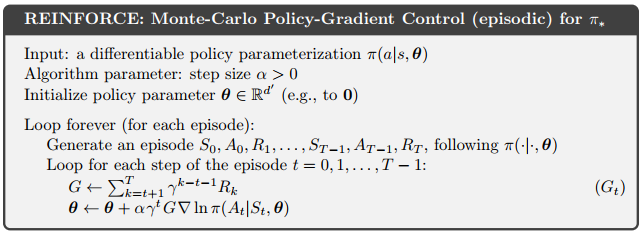
\includegraphics[width=0.7\textwidth] {Reinforce}}
\caption{REINFORCE Algorithm}\label{fig:reinforce}
\end{figure} 

\subsection{State-Based Baseline}
In order to reduce variance, we introduce a baseline to our gradient estimate. The addition of a state-based baseline $b(s)$ does not introduce bias into our estimate. That is, the gradient of the policy objective function $J(\theta)$ can be expressed as:
\begin{align*}
    \nabla_\theta J(\theta) = \BBE_{\tau \sim p_\theta} \left[\sum_{t=0}^{T-1} \nabla_\theta \log \pi_\theta(a_t \vert s_t) G_t\right] = \BBE_{\tau \sim p_\theta} \left[\sum_{t=0}^{T-1} \nabla_\theta \log \pi_\theta(a_t \vert s_t) (G_t - b(s_t))\right]
\end{align*}

In other words, $\BBE_{\tau \sim p_\theta} \left[\nabla_\theta \log \pi_\theta(a_t \vert s_t) b(s_t)\right] = 0$ for any $t$.


Before proving this we first show that
\begin{equation}\label{eq:baseline_proof_lemma}
    \int_{a_t} \pi_\theta(a_t \vert s_t) \nabla_\theta \log \pi_\theta(a_t \vert s_t) \, \da_t = 0
\end{equation}

\begin{tcolorbox}[breakable,enhanced,colback=gray!10!white,colframe=gray!50!black,
title={}]
\begin{align*}
\int_{a_t} \pi_\theta(a_t \vert s_t) \nabla_\theta \log \pi_\theta(a_t \vert s_t) \, \da_t &= \int_{a_t} \pi_\theta(a_t \vert s_t) \left(\frac{\nabla_\theta \pi_\theta(a_t \vert s_t)}{\pi_\theta(a_t \vert s_t)}\right) \, \da_t \\
&= \int_{a_t} \nabla_\theta \pi_\theta(a_t \vert s_t) \, \da_t \\
&= \nabla_\theta \int_{a_t} \pi_\theta(a_t \vert s_t) \, \da_t = \nabla_\theta \cdot 1 = 0
\end{align*}
\end{tcolorbox}
Next, consider the proof of $\BBE_{\tau \sim p_\theta} \left[\nabla_\theta \log \pi_\theta(a_t \vert s_t) b(s_t)\right] = 0$.
\begin{tcolorbox}[breakable,enhanced,colback=gray!10!white,colframe=gray!50!black,
title={$\BBE_{\tau \sim p_\theta} \left[\nabla_\theta \log \pi_\theta(a_t \vert s_t) b(s_t)\right] = 0$}]
\begin{align*}
&\BBE_{\tau \sim p_\theta} \left[\nabla_\theta \log \pi_\theta(a_t \vert s_t) b(s_t)\right] \\
%
&= \int p_\theta(\tau) \nabla_\theta \log \pi_\theta(a_t \vert s_t) b(s_t) \dtau \\
%
&= \int_{s_0} \int_{a_0} \cdots \int_{s_t} \int_{a_t} \cdots \int_{s_T} \mu(s_0) \pi_\theta(a_0 \vert s_0) \cdots P(s_t \vert s_{t-1}, a_{t-1}) \pi_\theta(a_t \vert s_t) \cdots P(s_T \vert s_{T-1}, a_{T-1}) \\
&\qquad \qquad \qquad \nabla_\theta \log \pi_\theta(a_t \vert s_t) b(s_t) \, \ds_0 \, \da_0 \cdots \ds_T \\
%
&= \int_{s_0} \cdots \int_{s_t} \int_{a_t} \mu(s_0) \cdots P(s_t \vert s_{t-1}, a_{t-1}) \pi_\theta(a_t \vert s_t) \nabla_\theta \log \pi_\theta(a_t \vert s_t) b(s_t) \\
&\qquad \qquad \qquad \cdots \int_{a_{T-1}} \pi_\theta(a_{T-1} \vert s_{T-1}) \underbrace{\int_{s_T} P(s_T \vert s_{T-1}, a_{T-1})\,\ds_T}_{=1} \, \da_{T-1} \cdots \, \da_0 \, \ds_0 \\
% 
&= \int_{s_0} \cdots \int_{s_t} \int_{a_t} \mu(s_0) \cdots P(s_t \vert s_{t-1}, a_{t-1}) \pi_\theta(a_t \vert s_t) \nabla_\theta \log \pi_\theta(a_t \vert s_t) b(s_t) \\
&\qquad \qquad \qquad \cdots  \underbrace{\int_{a_{T-1}} \pi_\theta(a_{T-1} \vert s_{T-1}) \, \da_{T-1}}_{=1} \,  \cdots \, \da_0 \, \ds_0 \\
% 
&= \int_{s_0} \int_{a_0} \cdots \int_{s_t} \int_{a_t} \mu(s_0) \pi_\theta(a_0 \vert s_0) \cdots P(s_t \vert s_{t-1}, a_{t-1}) \pi_\theta(a_t \vert s_t) \\
&\qquad \qquad \qquad \nabla_\theta \log \pi_\theta(a_t \vert s_t) b(s_t) \, \da_t \, \ds_t \cdots \da_0 \, \ds_0 \\
% 
&= \int_{s_0} \int_{a_0} \cdots \int_{s_t} \mu(s_0) \pi_\theta(a_0 \vert s_0) \cdots P(s_t \vert s_{t-1}, a_{t-1}) b(s_t) \\
&\qquad \qquad \qquad \underbrace{\int_{a_t} \pi_\theta(a_t \vert s_t) \nabla_\theta \log \pi_\theta(a_t \vert s_t) \, \da_t}_{=0 \text{ from~\eqref{eq:baseline_proof_lemma}}} \, \ds_t \cdots \da_0 \, \ds_0 \\
&=0
\end{align*}
\end{tcolorbox}
Thus, we have shown that \(\BBE_{\tau \sim p_\theta} \left[\nabla_\theta \log \pi_\theta(a_t \vert s_t) b(s_t)\right] = 0 \).

But why does it reduce the variance? Intuitively, by making the target values smaller (by subtracting the baseline), we are reducing the variance. To understand why the introduction of a baseline reduces variance, we consider informal reasoning by finding the baseline that minimizes the variance.

The variance \(\text{Var}(X)\) of a random variable \(X\) is defined as

\begin{align*}
\text{Var}(X) \triangleq \BBE[X^2] - \BBE[X]^2.
\end{align*}

We want to show that $\text{Var}(X) < \text{Var}(Y)$, where $X = \sum_{t=0}^{T-1} \nabla_\theta \log \pi_\theta(a_t \vert s_t) (G_t - b(s_t))   $, and $Y = \sum_{t=0}^{T-1} \nabla_\theta \log \pi_\theta(a_t \vert s_t) G_t$.

\vspace{10pt}
\textbf{Analysis 1. Finding the baseline that minimizes the variance} 


Let $X = \underbrace{\nabla_\theta \log \pi_\theta(a_t \vert s_t)}_{\triangleq \psi_t} (G_t - \underbrace{b(s_t)}_{\triangleq b_t})$

Now, let's consider the variance:
\begin{align*}
    \text{Var}(\psi_t (G_t - b_t)) = \BBE[(\psi_t (G_t - b_t))^2] - \BBE[\psi_t (G_t - b_t)]^2
\end{align*}

We showed that $\BBE[\psi_t (G_t - b_t)] = \BBE[\psi_t (G_t)]$, thus, the second term, \(\BBE[g_t (G_t - b_t)]^2\), does not depend on the choice of \(b_t\).
In order to minimize the variance, we need to find the optimal baseline \(b(s_t)\) that satisfies the condition \(\frac{d\text{Var}(\psi_t(G_t - b_t)}{db_t} = 0\). Differentiating with respect to \(b_t\) and setting it to zero, we obtain:

\[
\frac{d\text{Var}(\psi_t (G_t - b_t))}{db_t} = \frac{d}{db_t} \BBE[(\psi_t (G_t - b_t))^2] = \BBE[-2\psi_t^2 (G_t - b_t)] = 0
\]

Simplifying the equation, we find that:
\[
\BBE[\psi_t^2 G_t] = \BBE[\psi_t^2 b_t]
\]
This allows us to determine the optimal baseline \(b_t\) as:

\[
b_t = \frac{\BBE[(\nabla_\theta \log \pi_\theta(a_t \vert s_t))^2 G_t]}{\BBE[(\nabla_\theta \log \pi_\theta(a_t \vert s_t))^2]}
\]

While this expression provides a general formula for the optimal baseline, in practice, a common choice is to use the on-policy value function \(V_\pi(s_t)\) as the baseline.

\begin{itemize}
    \item Another informal reasoning can be found 
\href{https://danieltakeshi.github.io/2017/03/28/going-deeper-into-reinforcement-learning-fundamentals-of-policy-gradients/#:~:text=The%20variance%20is%20approximated%20as%3A
}{\underline{here}}.
    \item For a discussion on a more general form of a baseline see~\cref{section:GAE}.
\end{itemize}


\subsection{Vanilla Policy Gradient}

\begin{figure}[ht]
\center{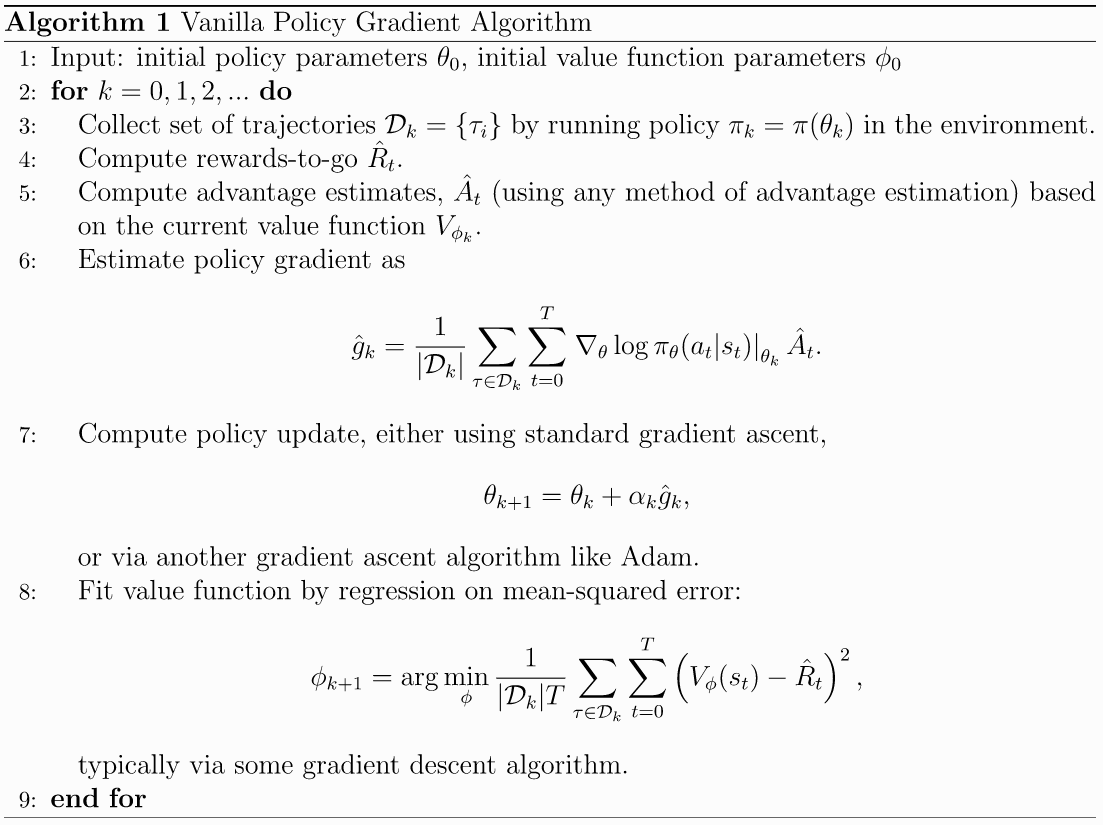
\includegraphics[width=0.7\textwidth] {Vanilla}}
\caption{Vanilla Policy Gradient Algorithm}\label{fig:vanilla}
\end{figure} 

\subsection{Off-Policy Policy Gradient Using Importance Sampling}\label{section:pg_off_policy}
Assume that instead of having samples collected under $\pi_\theta$, we have samples collected under another policy $\pi_\beta$. In this case, the policy gradient can be expressed in terms of the expectation over the trajectories under $\pi_\beta$ using importance sampling. First, for $t_2 \ge t_1$, define $w_{t_1 \to t_2}$ as
\begin{align}
w_{t_1 \to t_2} \triangleq \prod_{t= t_1}^{t_2}
    \frac{\pi_\theta(a_t \vert s_t)}{\pi_\beta(a_t \vert s_t)}.
\end{align}
Next, let $r(\tau)$ denote the sum of reward for trajectory $\tau$, then
\begin{align*}
    J(\theta) = \BBE_{\tau \sim p_\theta} [r(\tau)] = \BBE_{\tau \sim p_\beta} \left[\frac{p_\theta(\tau)}{p_\beta(\tau)} r(\tau) \right]
\end{align*}
where 
\begin{align*}
    \frac{p_\theta}{p_\beta} = \frac{\mu(s_0) \prod_{t=0}^{T-1}\pi_\theta(a_t \vert s_t) P(s_{t+1}\vert a_t, s_t)}{\mu(s_0) \prod_{t=0}^{T-1}\pi_\beta(a_t \vert s_t) P(s_{t+1}\vert a_t, s_t)} =
    \prod_{t=0}^{T-1}
    \frac{\pi_\theta(a_t \vert s_t)}{\pi_\beta(a_t \vert s_t)} = w_{0\to{T-1}}.
\end{align*}

Thus,
\begin{align}\label{eq:off_policy_pg_raw}
    \nabla_\theta J(\theta) = \BBE_{\tau \sim p_\beta} \left[w_{0 \to {T-1}} \left(\sum_{t=0}^{T-1} \nabla_\theta \log \pi_\theta(a_t\vert s_t)\right) \left(\sum_{t=0}^{T-1} r(s_t, a_t)\right) \right]
\end{align}
This version of off-policy policy gradient however have high variance.
From here forward, different works, make different estimations of~\eqref{eq:off_policy_pg_raw} in order to reduce the variance.

Causality trick 1: Current action cannot affect the past rewards. Thus, we change the trajectory reward to reward-to-go.

\begin{align*}
    \nabla_\theta J(\theta) &\approx \BBE_{\tau \sim p_\beta} \left[w_{0 \to {T-1}} \left(\sum_{t=0}^{T-1} \nabla_\theta \log \pi_\theta(a_t\vert s_t) \sum_{t^\prime=t}^T r(s_{t^\prime}, a_{t^\prime})\right) \right] \\
    &= \BBE_{\tau \sim p_\beta} \left[\left(\sum_{t=0}^{T-1} w_{0 \to {T-1}} \nabla_\theta \log \pi_\theta(a_t\vert s_t) \sum_{t^\prime=t}^{T-1} r(s_{t^\prime}, a_{t^\prime})\right) \right]\\
    &= \BBE_{\tau \sim p_\beta} \left[\left(\sum_{t=0}^{T-1} w_{0\to t} \nabla_\theta \log \pi_\theta(a_t\vert s_t) w_{{t+1} \to {T-1}} \sum_{t^\prime=t}^{T-1} r(s_{t^\prime}, a_{t^\prime})\right) \right]
    % &= \BBE_{\tau \sim p_\beta} \left[\left(\sum_{t=0}^{T-1} \left( \prod_{t^\prime=0}^{t}\frac{\pi_\theta(a_{t^\prime} \vert s_{t^\prime})}{\pi_\beta(a_{t^\prime} \vert s_{t^\prime})} \right) \nabla_\theta \log \pi_\theta(a_t\vert s_t) \left( \prod_{t^\prime=t+1}^{T-1}\frac{\pi_\theta(a_{t^\prime} \vert s_{t^\prime})}{\pi_\beta(a_{t^\prime} \vert s_{t^\prime})} \right) \sum_{t^\prime=t}^{T-1} r(s_{t^\prime}, a_{t^\prime})\right) \right]
\end{align*}

Causality trick 2: Future actions cannot affect the current reward. Thus, we drop the importance samplings into the future. First note that
\begin{align*}
    w_{{t+1} \to {T-1}} = \frac{w_{{0} \to {T-1}}}{w_{{0} \to {t}}}
\end{align*}

\begin{align}
\nabla_\theta J(\theta) &\approx \BBE_{\tau \sim p_\beta} \left[\left(\sum_{t=0}^{T-1} w_{0\to t} \nabla_\theta \log \pi_\theta(a_t\vert s_t)  \sum_{t^\prime=t}^{T-1} \frac{w_{{0} \to {T-1}}}{w_{{0} \to {t}}} r(s_{t^\prime}, a_{t^\prime})\right) \right]\nn\\
&\approx \BBE_{\tau \sim p_\beta} \left[\left(\sum_{t=0}^{T-1} w_{0\to t} \nabla_\theta \log \pi_\theta(a_t\vert s_t)  \sum_{t^\prime=t}^{T-1} \frac{w_{{0} \to {t^\prime}}}{w_{{0} \to {t}}} r(s_{t^\prime}, a_{t^\prime})\right) \right] \label{eq:off_policy_pg_after_causality1}
\end{align}

Introducing state-based baseline and discount factor to~\eqref{eq:off_policy_pg_after_causality1} yields
\begin{align}
\nabla_\theta J(\theta) &\approx \BBE_{\tau \sim p_\beta} \left[\left(\sum_{t=0}^{T-1} w_{0\to t}\gamma^t \nabla_\theta \log \pi_\theta(a_t\vert s_t)  \left(\sum_{t^\prime=t}^{T-1} \gamma^{t^\prime - t}\frac{w_{{0} \to {t^\prime}}}{w_{{0} \to {t}}} r(s_{t^\prime}, a_{t^\prime}) - b(s_t)\right)\right) \right],\label{eq:off_policy_pg_after_causality2}
\end{align}
which is the formulation in~\cite{precup2000eligibility}.

As before,~\eqref{eq:off_policy_pg_after_causality2} can have high variance due to having the multiplication of importance sampling fractions.
One approach to further reduce the variance is to make sure that the learned policy $\pi_\theta$ does not deviate too far from the behavior policy $\pi_\beta$, thus keeping the variance of the importance weights from becoming too large~\cite{levine2020offline}.
One way to achive this to introduce regulizer~\cite{levine2013guided,levine2020offline}:
\begin{align*}
\nabla_\theta J(\theta) &\approx \BBE_{\tau \sim p_\beta} \left[\left( w_{{0} \to {T-1}} \sum_{t=0}^{T-1}\gamma^t \nabla_\theta \log \pi_\theta (a_t\vert s_t) \hat A(s_t,a_t)\right) + \lambda \log w_{{0} \to {T-1}}\right].
\end{align*}
This regulizer which is the softmax over the importance weight, adjust the policy $\pi_\theta$ to ensure that at least one sample has a high importance weight.

\subsection{Policy Gradient Implementation Notes}

\begin{enumerate}
    \item \textcolor{red}{with Automatic Differentiation Tools}
    \item \textcolor{red}{On normalization}
\end{enumerate}

\newpage
\section{Actor-Critic}

Another way to reduce variance in policy gradient methods is to use a bootstrapping target. If we replace the advantage function in Vanilla policy gradient with a TD(0)-like target, we obtain the actor-critic algorithm, which reduces the variance at the cost of introducing bias. Similar to the Vanilla policy gradient method, the actor-critic algorithm consists of two networks: one for value-function approximation and one for policy. The difference is that in Vanilla PG, we only use the value network for the baseline, whereas in the actor-critic algorithm, we also use the same network to estimate the return. The policy network is referred to as \textit{the actor} since it interacts with the environment, while the value network, \textit{the critic}, maintains the value of the actions taken by the actor.

\subsection{Actor-Critic Derivation}

The policy gradient expression
\begin{align*}
    \nabla_\theta J(\theta) = \BBE_{\tau \sim p_\theta} \left[\sum_{t=0}^{T-1} \nabla_\theta \log \pi_\theta(a_t \vert s_t) G_t\right],
\end{align*}
can be interpreted as a weighted version of the maximum likelihood objective, with the weights being the single-sample reward-to-go. In other words, policy gradient increases or decreases the likelihood of an action depending on the value of its single-sample reward-to-go. Compare this to behavioral cloning, where the likelihood of all actions in a given dataset is increased irrespective of their corresponding reward-to-go:
\begin{align*}
    \nabla_\theta J_{\rm {BC}}(\theta) = \BBE_{\tau \sim p_\beta} \left[\sum_{t=0}^{T-1} \nabla_\theta \log \pi_\theta(a_t \vert s_t)\right].
\end{align*}
However, one way to reduce the variance in policy gradient is to replace the single-sample reward-to-go with the expected return given the state and action. That is

\begin{align*}
    \nabla_\theta J(\theta) &= \BBE_{\tau \sim p_\theta} \left[\sum_{t=0}^{T-1} \nabla_\theta \log \pi_\theta(a_t \vert s_t) \BBE_\pi[G_t \vert s_t, a_t]\right] \\
    &= \BBE_{\tau \sim p_\theta} \left[\sum_{t=0}^{T-1} \nabla_\theta \log \pi_\theta(a_t \vert s_t) Q^\pi(s_t,a_t)\right]\\
    &= \BBE_{\tau \sim p_\theta} \left[\sum_{t=0}^{T-1} \nabla_\theta \log \pi_\theta(a_t \vert s_t) \left[R(s_t, a_t)+ \BBE_{s_{t+1}\sim P(s_{t+1}\vert s_t, a_t)}[V^\pi(s_{t+1})]\right]\right].
\end{align*}
Now we make an approximation and we replace $\BBE_{s_{t+1}\sim P(s_{t+1}\vert s_t, a_t)}[V^\pi(s_{t+1})]$ by $V^\pi(s_{t+1})$, meaning that we consider a single-sample estimate for $V^\pi(s_{t+1})$. Note, however, that we are making the single-sample estimate only for one timestep. Since, after one timestep, at $s_{t+1}$, since we are using $V^\pi(s_{t+1})$, we are going to be under $\BBE_\pi$ thereafter. \textbf{This will introduce bias at the cost of lower variance}. The modified policy gradient then becomes
\begin{align*}
    \nabla_\theta J(\theta) &= \BBE_{\tau \sim p_\theta} \left[\sum_{t=0}^{T-1} \nabla_\theta \log \pi_\theta(a_t \vert s_t) \left[R(s_t, a_t)+ V^\pi(s_{t+1})\right]\right].
\end{align*}

To obtain the actor-critic method, we introduce the state-base baseline and discount factor, $V^\pi(s_t)$ and $\gamma$ and we define the estimate of the advantage at time step $t$, denoted as $\hat{A}_t$, as

$$\hat{A}_t = \underbrace{R(s_t,a_t) + \gamma V_\phi^\pi(s_{t+1})}_{\text{return estimator}} - \underbrace{V_\phi^\pi(s_t)}_{\text{baseline}},$$
and
\begin{align*}
    \nabla_\theta J(\theta) &= \BBE_{\tau \sim p_\theta} \left[\sum_{t=0}^{T-1} \nabla_\theta \log \pi_\theta(a_t \vert s_t) \hat A_t \right].
\end{align*}

This forms the basis of the online actor-critic algorithm.

\begin{figure}[ht]
\center{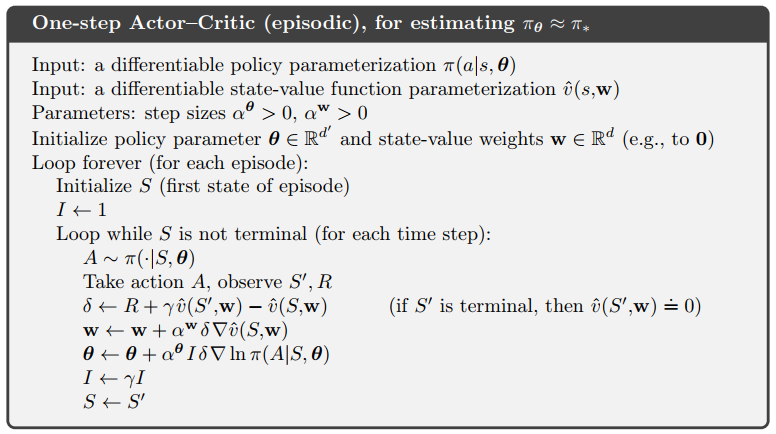
\includegraphics[width=0.7\textwidth] {Online_actor_critic}}
\caption{Online Actor-Critic Algorithm}\label{fig:onlice_actor_critic}
\end{figure} 
% 
\begin{center}
\begin{tcolorbox}
[breakable,enhanced,colback=purple!10!white,colframe=purple!30!black,
title={Batch actor-critic algorithm},width=0.7\linewidth]
\begin{enumerate}[\hspace{1cm}(1)]
    \item Sample $\{s_i,a_i,s_i',r_i\}$ under $\pi_\theta(a|s)$ (run the agent on the environment)
    \item Fit $\hat{V}_\phi^\pi(s)$ to sampled reward sum or TD
    \item Evaluate $\hat{A}^\pi(s_i,a_i) = r(s_i,a_i) + \hat{V}_\phi^\pi(s_i') - \hat{V}_\phi^\pi(s_i)$
    \item Update $\theta$ using $\nabla_\theta J(\theta) \approx \sum_i \nabla_\theta \log\pi_\theta(a_i|s_i)\hat{A}^\pi(s_i,a_i)$
    \item Go back to step 1
\end{enumerate}
\end{tcolorbox}
\end{center}

This represents the Batch actor-critic algorithm, where the agent collects a batch of samples from the environment, updates the value function approximation, evaluates the advantage function, and performs a policy update using the policy gradient. The process is repeated iteratively to improve the policy and value function estimates.

\subsection{Discount Factor}
The discount factor introduces changes to the original MDP (with the transition dynamics $p(s^\prime\vert s, a)$), altering it into another MDP depicted in Figure~\ref{fig:discount_factor}. This modified MDP incorporates a "death" state, denoted as $s_\rmd$, which corresponds to adjusted transition dynamics $\tilde p(s^\prime\vert s, a)$ defined as:
\begin{align*}
\tilde p(s^\prime \vert s,a) = 
    \begin{cases}
        1 - \gamma, \qquad \qquad &\mbox{if } s^\prime = s_\rmd\\
        \gamma p(s^\prime \vert s, a), \qquad\qquad &\mbox{else.} 
    \end{cases}
\end{align*}
Given this adjusted MDP (Figure~\ref{fig:discount_factor}), we express the value function $V_\pi(s)$ as follows:
\begin{align*}
    V_\pi(s) &= \BBE_{a\sim\pi(a\vert s)}\left[ r(s,a) + \BBE_{s^\prime \sim \tilde p(s^\prime \vert s, a)}[V_\pi(s^\prime)]\right]\\
    &= \BBE_{a\sim\pi(a\vert s)}\left[ r(s,a) + \gamma \BBE_{s^\prime \sim p(s^\prime \vert s, a)}[V_\pi(s^\prime)] + (1 - \gamma)(\underbrace{V_\pi(s_\rmd)}_{=0}) \right]\\
    &= \BBE_{a\sim\pi(a\vert s)}\left[ r(s,a) + \gamma\BBE_{s^\prime \sim p(s^\prime \vert s, a)}[ V_\pi(s^\prime)]\right]
\end{align*}
The policy gradient for this modified MDP, after applying the causality trick, can be approximated as
\begin{align}
\nabla_\theta J(\theta) &\approx \BBE_{\tau\sim p_\theta}\left[\sum_{t=0}^{T-1} \nabla_\theta \log \pi_\theta(a_t \vert s_t) \left(\sum_{t^\prime = t}^{T-1} \gamma ^{t^\prime}r(s_t, a_t)\right) \right]\nn\\
&= \BBE_{\tau\sim p_\theta}\left[\sum_{t=0}^{T-1} \gamma ^{t }\nabla_\theta \log \pi_\theta(a_t \vert s_t) \left(\sum_{t^\prime = t}^{T-1} \gamma ^{t^\prime -t}r(s_t, a_t)\right) \right]\label{eq:discount_factor_pg_1}
\end{align}
This is similar to the~\eqref{eq:off_policy_pg_after_causality2} with $\beta = \theta$. The interpretation of Equation~\eqref{eq:discount_factor_pg_1} is that the introduction of the death state (due to the discount factor) results in reduced importance assigned to both future rewards and future decisions. In essence, making the correct decision sooner becomes more critical, and the impact of $\nabla_\theta \log \pi_\theta(a_t \vert s_t)$ diminishes as $t$ increases.

However, in practice, we commonly omit the $\gamma^t$ term, leading to the use of the following policy gradient approximation:

\begin{align}
\nabla_\theta J(\theta) &\approx \BBE_{\tau\sim p_\theta}\left[\sum_{t=0}^{T-1} \nabla_\theta \log \pi_\theta(a_t \vert s_t) \left(\sum_{t^\prime = t}^{T-1} \gamma ^{t^\prime -t}r(s_t, a_t)\right) \right]\label{eq:discount_factor_pg_2}
\end{align}

Based on Equation~\eqref{eq:discount_factor_pg_2}, the sole alteration in the actor-critic formulation lies in the computation of $\hat{A}^\pi(s,a)$, which is expressed as:

\begin{align*}
    \hat{A}^\pi(s,a) = r(s,a) + \gamma \hat{V}_\phi^\pi(s^\prime) - \hat{V}_\phi^\pi(s_i)
\end{align*}

\begin{figure}[ht]
\center{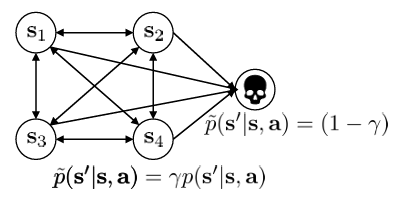
\includegraphics[width=0.3\textwidth] {Discount_Factor}}
\caption{MDP with Discount Factor}\label{fig:discount_factor}
\end{figure}

\subsection{Off-Policy Actor-Critic}
\begin{itemize}
    \item Transitions ($s_i, a_i, r_i, s^\prime_i)$ under any policy is stored in the replay buffer. Define $a_i^\pi \triangleq \pi_\theta(s_i)$.
    \item On-policy actor-critic has two limitations for being used as an off-policy algorithm:
    \begin{enumerate}
        \item In the actor-critic derivation, we replaced $\BBE_\pi[V^\pi(s^\prime)]$ with the single-sample estimate $V^\pi(s^\prime)$. This replacement was sort of valid as long as we at least sample under the same policy. Thus, we cannot use the transition $(s,a,s^\prime, r)$ from the replay buffer which was collected under another policy to update the value function (the critic update).
        However, if we instead use $Q$ values. Then, we can use the transition $(s,a,s^\prime, r)$ to update the $\hat Q_\phi^\pi$ values.        
        \item For the same reason, during the actor update, we are interested in updating the chance of selecting an action, based on the value of that action. Thus, we require to update the action that current policy would have chosen at state $s$, which is $\pi_\theta(s)$, and not the action $a$ from the transition.
    \end{enumerate}
    
    \item To train the actor we completely ignore the transition from the buffer, we only use $s_i$. The reason is that the reward $r_i$ in the buffer is the reward collected under $a_i$. However, the current policy takes action $a_i^\pi$, for which we don't know the reward to be collected. However, we can estimate the reward-to-go using the critic network $\hat Q_\phi^\pi$. We want to know how good is the action that we would have taken under current policy if we were at $s_i$.
    \item Note that we removed the baseline from the Actor Target. 
    \end{itemize}

\begin{figure}[ht]
\center{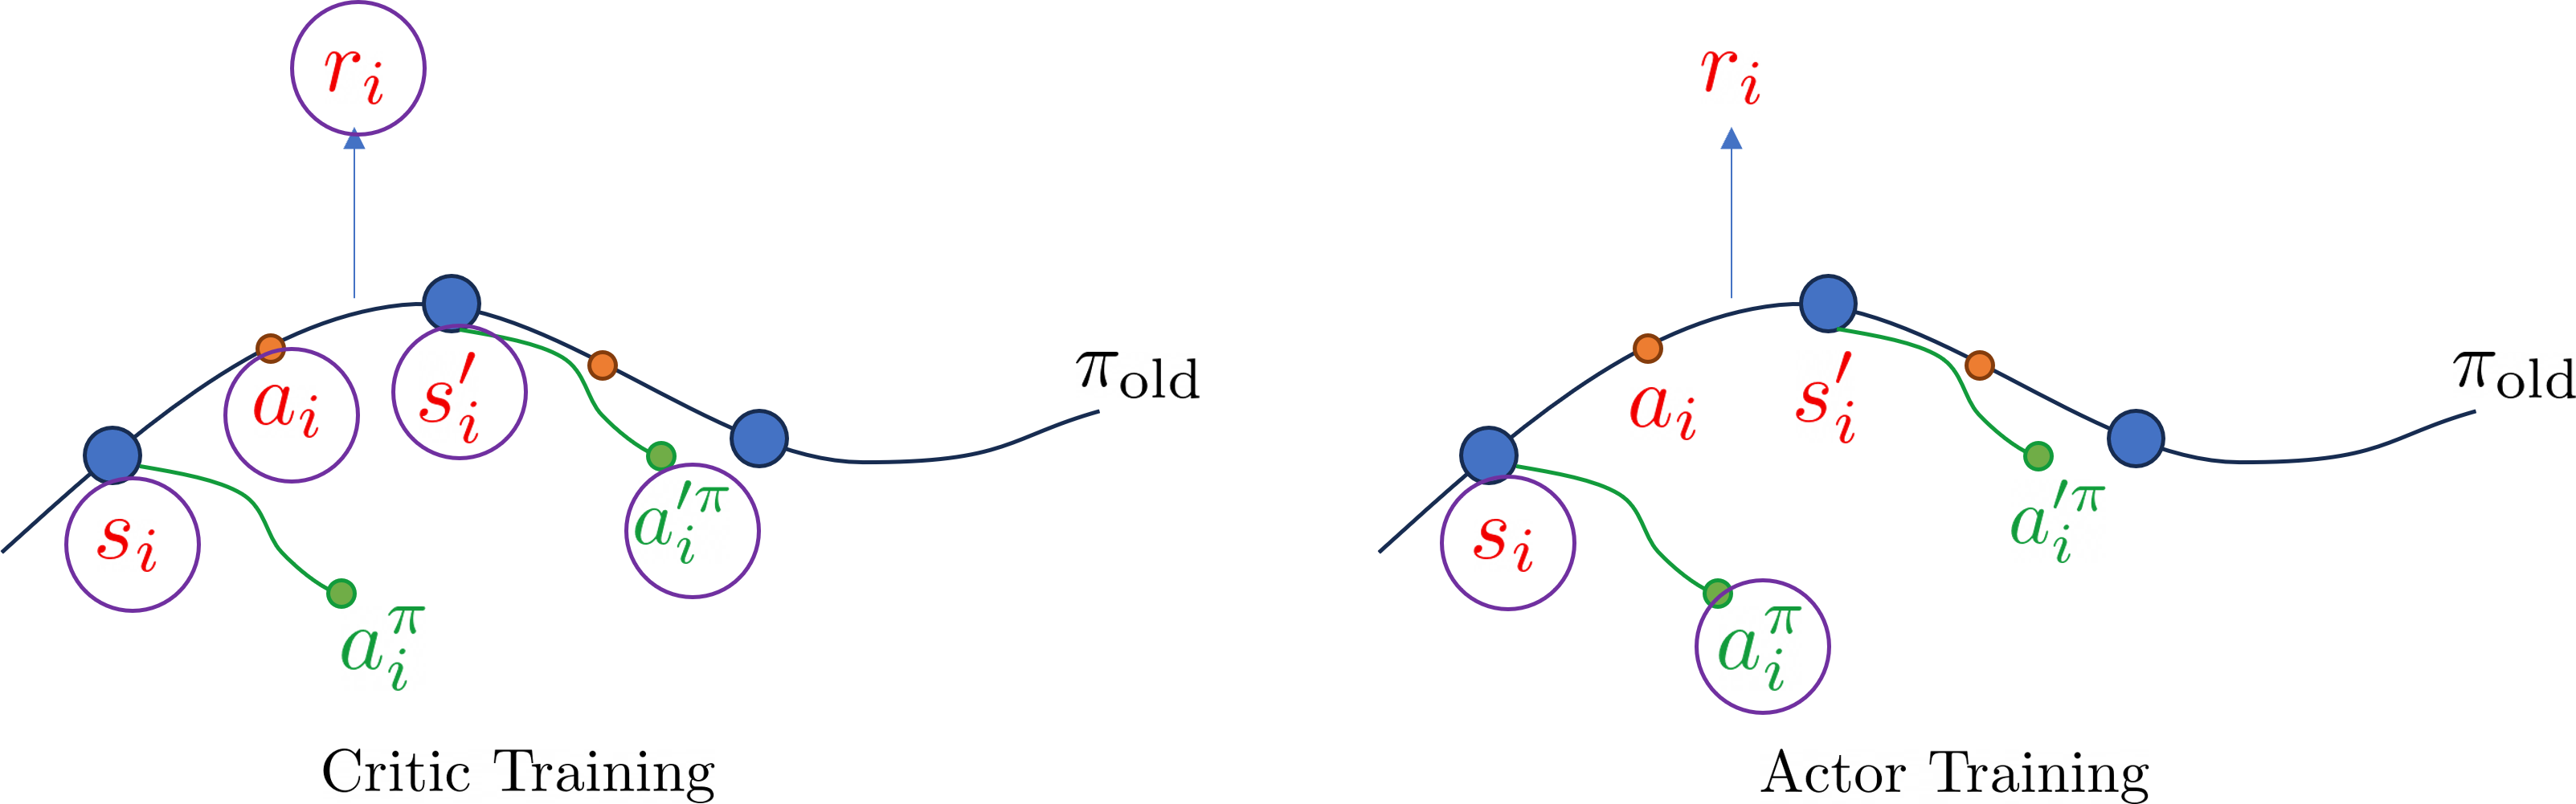
\includegraphics[width=0.9\textwidth] {Off_policy_Actor_critic}}
\caption{Off-Policy Actor-Critic Training}\label{fig:off_policy_actor_critic}
\end{figure} 


\begin{table}[ht]
    \centering
    \renewcommand{\arraystretch}{2}
    \begin{tabular}{c|c|c}        
         & \textbf{On-Policy} & \textbf{Off-Policy} \\        
         \hline
        \textbf{Networks} & $\hat V_\phi^\pi, \pi_\theta$& $\hat Q_\phi^\pi, \pi_\theta$ \\        
        \textbf{Critic Target} & $\hat V_\phi^\pi(s_i) \gets r_i + \gamma \hat V_\phi^\pi(s^\prime_i)$ &  $\hat Q_\phi^\pi(s_i, a_i) \gets r_i + \gamma \hat Q_\phi^\pi(s^\prime_i, a_i^{\prime\pi})$\\       
        % \textbf{Actor Target} & $r_i + \gamma \hat V_\phi^\pi (s_i^\prime) - \hat V_\phi^\pi(s_i)$ & $\hat Q_\phi^\pi(s_i, a_i^\pi) -\hat V_\phi^\pi(s_i)$\\
        \textbf{Actor Grad} & $\frac{1}{N}\sum_i \nabla_\theta \log \pi_\theta(a_i \vert s_i) \hat A_\phi^\pi(s_i, a_i)$ & $\frac{1}{N}\sum_i \nabla_\theta \log \pi_\theta(a_i^\pi \vert s_i) \hat Q_\phi^\pi(s_i, a_i^\pi)$ \\        
    \end{tabular}
    \caption{On-Policy vs. Off-Policy Actor-Critic}
    \label{tab:my_table}
\end{table}


\subsection{Actor-critic implementation notes}

\begin{itemize}
\item In theory, we should perform value function regression every time we update our policy to match the new policy's behavior. However, in practice, this can be computationally expensive. Therefore, we may instead take a few gradient steps at each iteration.
\item Since our target values are based on the old value function, we need to update the targets (i.e., $r + \gamma V(s')$) with the updated value function. This can be done by following these steps:
\begin{enumerate}
\item Update targets with current value function.
\item Regress onto targets to update the value function by taking a few gradient steps.
\item Repeat steps 1 and 2 several times.
\end{enumerate}
\item The process of fitting the value function critic is an iterative process where we alternate between computing target values and updating the value function to match the targets. This iterative process is crucial for training the critic network.
\item In regular policy gradient methods, it is necessary to visit a state multiple times to have a good estimate of the return. However, in actor-critic methods, even if the exact same state is not visited multiple times, there may be other similar states visited in different trials. As a result, the function approximator can capture some shared information between these states, leading to a better estimate of the expected return compared to a single-sample Monte Carlo update. However, this estimate is not as accurate as repeatedly visiting the exact same state and taking multiple trials from it, but it still provides some benefit.
\end{itemize}

\newpage

\section{Algorithms}
\subsection{GAE: Generalized Advantage Estimation}\label{section:GAE}
\href{https://arxiv.org/abs/1506.02438}{\underline{Link to paper}} | \href{https://arxiv.org/abs/1506.02438}{\underline{Link to code ADD}} 

\vspace{10pt}
Consider the definitions in~\Cref{fig:gae_summary}, and the following definition.

\begin{figure}[h]
    \centering
    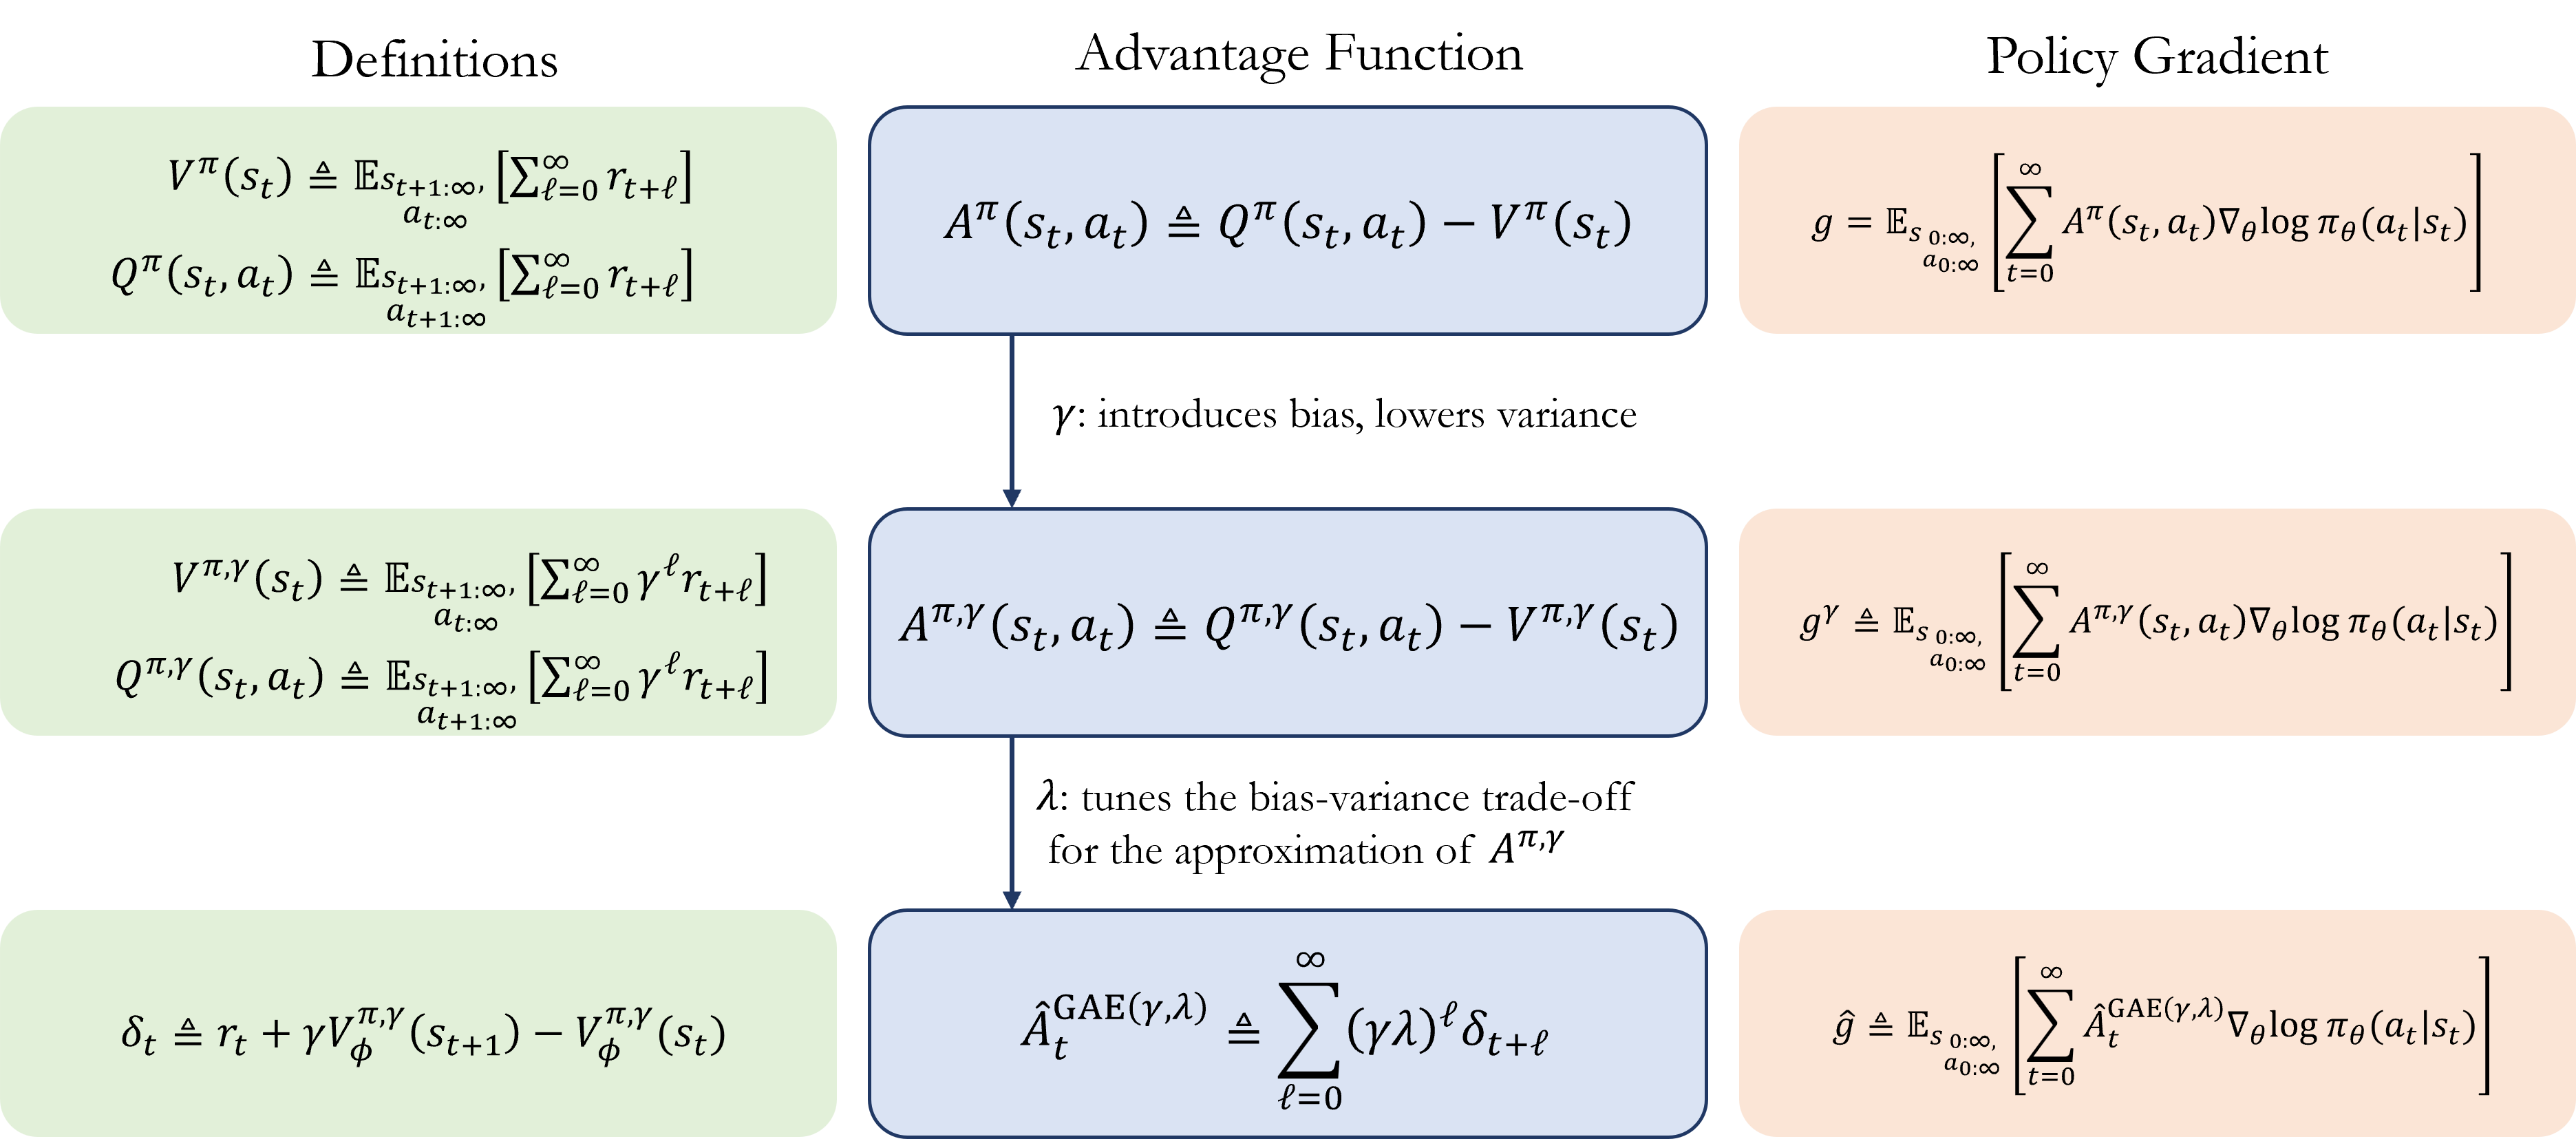
\includegraphics[width=1.0\linewidth]{Figures/GAE_table.png}
    \caption{Advantage functions definitions and their associated policy gradients}
    \label{fig:gae_summary}
\end{figure}

\begin{definition} 
The estimator $\hat{A}_t$ is $\gamma$-just if
\begin{align*}
\mathbb{E}_{s_{0:\infty} a_{0:\infty}} [\hat{A}_t(s_{0:\infty}, a_{0:\infty}) \nabla_{\theta} \log \pi_{\theta}(a_t | s_t) ] &= \mathbb{E}_{s_{0:\infty} a_{0:\infty}} [A_{\pi,\gamma}(s_t, a_t) \nabla_{\theta} \log \pi_{\theta}(a_t | s_t)].
\end{align*}
\end{definition}

A $\gamma$-just advantage function estimator $\hat{A}$ has the property that when it is substituted in place of $A{\pi,\gamma}$ in the policy gradient, it does not introduce any additional bias.

With these definitions, we can present \Cref{prop:GAE_prop}, which give a sufficient condition for $\hat A$ to be $\gamma$-just.

\begin{proposition}\label{prop:GAE_prop}
    Suppose that $\hat A_t$ can be written in the form $\hat A_t(s_{0:\infty},a_{0:\infty}) = Q_t(s_{t:\infty},a_{t:\infty}) - b_t(s_{0:t},a_{0:t-1})$ such that for all $(s_t,a_t)$, $\BBE_{s_{t+1:\infty}, a_{t+1:\infty}\vert {s_t, a_t}}[Q_t(s_{t:\infty},a_{t:\infty})] = Q^{\pi, \gamma}(s_t, a_t)$. Then, $\hat A$ is $\gamma$-just.
\end{proposition}
See \cite{schulman2015high} for the proof.

\Cref{prop:GAE_prop} shows that an advantage estimator $\hat{A}_t$ will be $\gamma$-just if it is composed of two terms - a state-dependent baseline $b_t$ and a $\gamma$-discounted Q-function estimator $Q_t$. Critically, $b_t$ can only depend on past and current states and past actions while $Q_t$ can depend on the full trajectory.

This implies we can reduce policy gradient variance by subtracting any function of past and current states and past actions as a baseline, without introducing bias.


\textbf{Objectives:}

The paper has two main objectives:

\begin{enumerate}
\item Provide an intuition for a variance reduction scheme in policy gradients.

\item Introduce an advantage function estimator that allows tuning the bias-variance tradeoff using two parameters $\gamma$ and $\lambda$.

\end{enumerate}

\textbf{Approach:}

The GAE aims to find a lower variance approximation to the true advantage function $A^{\pi}$. It does this in two main ways:

\begin{enumerate}
\item Introducing a discount factor $\gamma$ decreases variance at the cost of some bias. The GAE tries to estimate the $\gamma$-discounted advantage $A^{\pi,\gamma}$.

\item The parameter $\lambda$ controls the bias-variance tradeoff in the GAE estimator. Setting $\lambda=1$ gives an unbiased estimate of $A^{\pi,\gamma}$, while lower $\lambda$ reduces variance further but introduces some bias.
\end{enumerate}

In summary, the GAE provides an advantage function estimator with two knobs - $\gamma$ and $\lambda$ - to tune the bias-variance tradeoff. This enables constructing policy gradient algorithms with reduced variance.
In this method,
\begin{itemize}
    \item GAE uses $V_\phi^{\pi, \gamma}$, the value function estimator, instead of the ground-truth $V^{\pi,\gamma}$
    \item $\gamma$ controls the bias in $A^{\pi, \gamma}$ with respect to $A^\pi$. $A^{\pi, \gamma}$ is an unbiased estimator of $A^\pi$ for $\gamma =1$. Even with an accurate value function, setting $\gamma < 1$ introduces bias into the estimate. 
    \item $\lambda$ controls the bias in $\hat A_t^{\rm{GAE}(\gamma, \lambda)}$ with respect to $A^{\pi, \gamma}$. $\hat A_t^{\rm{GAE}(\gamma, \lambda)}$ is an unbiased estimator of $A^{\pi, \gamma}$ for $\lambda = 1$, regardless of the accuracy of the function approximator (will be described). In contrast, $\lambda < 1$ introduces bias only when the value function is inaccurate.
    \item Empirically, the paper suggests that the optimal value for $\lambda$ is much lower than the optimal value for $\gamma$. This difference is likely because $\lambda$ introduces less bias than $\gamma$, especially when the value function is reasonably accurate.
    \item Increasing either $\lambda$ or $\gamma$ reduces bias, but they do so toward different targets, and this reduction in bias comes at the cost of increased variance.
\end{itemize}

\textbf{GAE Advantage Function:}

GAE advantage function is equivalent to TD($\lambda$), which is the weighted-sum $n$-step TD errors, weighted by, $\lambda^n$, with $V_\phi^{\pi, \gamma}$ being the value function approximator. Consider the following defintions:
\begin{align*}
    \delta_t &\triangleq r_t + \gamma V_\phi^{\pi, \gamma}(s_{t+1}) - V_\phi^{\pi, \gamma}(s_t),\\
    \hat A_t^{(k)} &\triangleq \sum_{\ell=1}^{k-1} \gamma^{\ell} r_{t+\ell} + \gamma^k V_\phi^{\pi, \gamma}(s_{t+k}) - V_\phi^{\pi, \gamma}(s_t) = \sum_{\ell =0}^{k-1} \gamma^\ell \delta_{t+\ell}.\\
    % \left( \hat A_t^{(1)} + \lambda \hat A_t^{(2)} + \lambda^2 \hat A_t^{(3)} + \cdots \right)
\end{align*}
\begin{itemize}
     \item Infinite-horizon Case:
\end{itemize}

\begin{align*}
    \hat A_t^{\rm{GAE}(\gamma,\lambda)} &\triangleq (1-\lambda) \sum_{\ell = 0}^\infty \lambda^{\ell} \hat A_t^{(\ell + 1)}  = \sum_{\ell = 0}^\infty (\gamma \lambda)^{\ell} \delta_{t+\ell}
\end{align*}
It can be shown from the above definition that the following holds:
\begin{align*}
     \hat A_t^{\rm{GAE}(\gamma,\lambda)} = \frac{1}{1-\lambda}\delta_t + \gamma \lambda \hat A_{t+1}^{\rm{GAE}(\gamma,\lambda)}
\end{align*}

Note that 
\begin{align*}
    \hat A_t^{\rm{GAE}(\gamma,1)} &= \sum_{\ell = 0}^\infty \gamma^\ell \delta_{t+\ell} = \sum_{\ell = 0}^\infty \gamma^\ell r_{t+\ell} - V_\pi^{\pi, \gamma}(s_t)\\
    \hat A_t^{\rm{GAE}(\gamma,0)} &= \delta_t
\end{align*}
Thus, $\rm{GAE}(\gamma, 1)$ is $\gamma$-just regardless of accuracy of $V_\phi^{\pi, \gamma}$.

\begin{itemize}
     \item Finite-horizon Case:
\end{itemize}
\begin{align*}
\hat{A}_t^{\rm GAE} = \delta_t + (\gamma \lambda) \delta_{t+1} + (\gamma \lambda)^2 \delta_{t+2} + \ldots + (\gamma \lambda)^{T-t-1} \delta_{T-1},
\end{align*}
and
\begin{align*}
    \hat A_t^{\rm{GAE}(\gamma,\lambda)} &\triangleq \frac{1 - \lambda}{1 - \lambda^T} \sum_{\ell=0}^{T-1} \lambda^\ell \hat A_t^{(\ell+1)} = \frac{1}{1 - \lambda^T}\sum_{\ell=0}^{T-1} (\gamma \lambda)^\ell \left(1 - \lambda^{T-\ell}\right)\delta_{t+\ell}
\end{align*}



\newpage
\section{Appendix: Basic Statistics}\label{apx:basic_statistics}

\begin{itemize}
  \item \textbf{Probability:}
  \begin{itemize}
    \item $P(X)$ represents the probability of event $X$, ranging from 0 to 1.
    \item $X'$ denotes the complement of event $X$, such that $P(X') = 1 - P(X)$.
    \item $X \cup Y$ signifies the union of events $X$ and $Y$, with $P(X \cup Y) = P(X) + P(Y) - P(X \cap Y)$.
  \end{itemize}

  \item \textbf{Probability Properties:}
  \begin{itemize}
    \item \textbf{Marginal Probability:}
    \begin{itemize}
      \item For joint probability distribution $P(X, Y)$, the marginal probability of $X$ is obtained by summing or integrating over all possible values of $Y$: $P(X) = \int P(X, y) dy$.
    \end{itemize}
    \item \textbf{Conditional Probability:}
    \begin{itemize}
      \item $P(X|Y) = \frac{P(X \cap Y)}{P(Y)}$ denotes the conditional probability of $X$ given $Y$.
    \end{itemize}
    \item \textbf{Independence:}
    \begin{itemize}
      \item Events $X$ and $Y$ are independent if $P(X \cap Y) = P(X) \cdot P(Y)$.
    \end{itemize}
    \item \textbf{Law of Total Probability:}
    \begin{itemize}
      \item $P(A) = \sum_{i} P(A|B_i) \cdot P(B_i)$ for mutually exclusive and exhaustive events $B_1, B_2, \ldots$.
    \end{itemize}
  \end{itemize}

  \item \textbf{Expectation:}
  \begin{itemize}
    \item $\BBE(X)$ or $\mu$ represents the expectation of random variable $X$.
    \begin{itemize}
      \item For discrete $X$: $\BBE(X) = \sum_{x} x \cdot P(X = x)$.
      \item For continuous $X$ with probability density function $f(x)$: $\BBE(X) = \int x \cdot f(x) dx$.
    \end{itemize}
    \item \textbf{Linearity of Expectation:}
    \begin{itemize}
      \item $\BBE(aX + bY) = a\BBE(X) + b\BBE(Y)$ for random variables $X$ and $Y$, and constants $a$ and $b$.
    \end{itemize}
    \item \textbf{Law of the Unconscious Statistician:}
    \begin{itemize}
      \item $\BBE(g(X)) = \sum_{x} g(x)P(X=x)$, where $P(X=x)$ is the probability mass function of $X$.
    \end{itemize}
    \item \textbf{Importance Sampling:}
    \begin{itemize}
      \item $\BBE_{x\sim p(x)}[f(x)] = \BBE_{x\sim q(x)}\left[\frac{p(x)}{q(x)}f(x)\right]$.
      
    \end{itemize}
    
  \end{itemize}

  \item \textbf{Variance:}
    \begin{itemize}
    \item The variance of random variable $X$, denoted as $\text{Var}(X)$ or $\sigma^2$, measures the spread of $X$ around its expected value:
    \[
    \text{Var}(X) = E[(X - E(X))^2] = E(X^2) - [E(X)]^2
    \]    

        \item \textbf{Covariance:}
        \begin{itemize}
            \item $\text{Cov}(X, Y) = E[(X - E(X))(Y - E(Y))]$ measures the linear relationship between random variables $X$ and $Y$.
        \end{itemize}
        \item \textbf{Conditional Expectation:}
        \begin{itemize}
            \item $\BBE(X|Y=y) = \sum_{x} x \cdot P(X = x|Y = y)$ for discrete $X$ and $Y$, and $\BBE(X|Y=y) = \int x \cdot f(x|y) dx$ for continuous $X$ and $Y$ with conditional probability density function $f(x|y)$.
        \end{itemize}        
        \item \textbf{Law of Iterated Expectations:} 
        \begin{itemize}
            \item $\BBE(E(X|Y)) = E(X)$.
        \end{itemize}

    
    \end{itemize}
    

\end{itemize}

\bibliographystyle{elsarticle-num} 
\bibliography{policy_gradient} 

\end{document}